\documentclass[aspectratio=169]{beamer}
\usepackage[T1]{fontenc}
\usepackage[english]{babel}

\usetheme{Madrid}
\usecolortheme{default}

% \usepackage[utf8]{inputenc}
\usepackage[utf8]{vietnam}
\usepackage{amsmath, amssymb, amsfonts}
\usepackage{algorithm}
\usepackage[noend]{algpseudocode}
\usepackage{svg}
\usepackage{csquotes}
\usepackage{ragged2e}

\beamertemplatenavigationsymbolsempty

\usepackage[backend=biber, defernumbers=true,style=authortitle-ibid,citetracker=true,maxnames=1, minnames=1,sorting=none,doi=false,url=false]{biblatex}

\renewcommand*{\bibfont}{\normalfont\small}

\addbibresource{all-ref.bib}

\title[SAAS]{Giải thuật đàn kiến tự thích ứng cho bài toán điều hướng thu thập}
\author[Việt, Vũ]{Lê Thế Việt - 20520093, Huỳnh Hoàng Vũ - 20520864}
\date[January 2024]{
    Giảng viên hướng dẫn: TS. Lương Ngọc Hoàng \\
    \vspace{0.3cm}
    January, 2024}
\institute[UIT]
{
    Vietnam National University, Ho Chi Minh City - University of Information Technology \\
    \vspace{0.2cm}
    
\includegraphics[scale=0.135]{img/Logo_UIT_updated.jpg}
}
% \AtBeginSection[]
% {
%   \begin{frame}
%     \frametitle{Table of Contents}
%     \tableofcontents[currentsection]
%   \end{frame}
% }

\AtBeginSection[]{
\begin{frame}
    \tableofcontents[sectionstyle=show/shaded, subsectionstyle=show/shaded/hide, subsubsectionstyle=show/shaded/hide]
\end{frame}
}
\AtBeginSubsection[]{
\begin{frame}
    \tableofcontents[sectionstyle=show/shaded, subsectionstyle=show/shaded/hide, subsubsectionstyle=show/shaded/hide]
\end{frame}
}
\begin{document}
\maketitle
\begin{frame}{Our Publication}
    \justifying
    Vu Hoang Huynh, The Viet Le and Ngoc Hoang Luong. “Self-Adaptive Ant System with Hierarchical Clustering for the Thief Orienteering Problem”. In: Proceedings of the 12th International Symposium on Information and Communication Technology. SOICT 2023. ACM, Dec. 2023.
\end{frame}

\begin{frame}
    \frametitle{Table of Contents}
    \tableofcontents[sectionstyle=show, subsectionstyle=hide, subsubsectionstyle=hide]
\end{frame}

\section{Problem Definition}
\begin{frame}{Problem description}
    % \hspace{0.1cm}
    \vspace*{-0.25cm}
    \begin{block}{Thief Orienteering Problem (ThOP)}
        \footnotesize ThOP\footnotemark is a \textbf{multi-component optimization problem}, it combines the \textbf{Orienteering Problem (OP)} and \textbf{Knapsack Problem (KP)}.
    \end{block}
    \footnotetext{\fullcite{8477853}}
\end{frame}

\begin{frame}{Problem description}
    % \hspace{0.1cm}
    \onslide<1->{
        \begin{columns}
            \hspace{0.17cm}
            \begin{column}{0.55\textwidth}
                \begin{block}{Orienteering problem (OP)}
                    \justifying
                    \footnotesize OP is a \textbf{routing problem} in which the goal is to determine a path through a given set of points of interest that \textbf{maximizes a total score} while \textbf{satisfying a given time budget}.
                \end{block}
            \end{column}

            \begin{column}{0.45\textwidth}
                \begin{center}
                    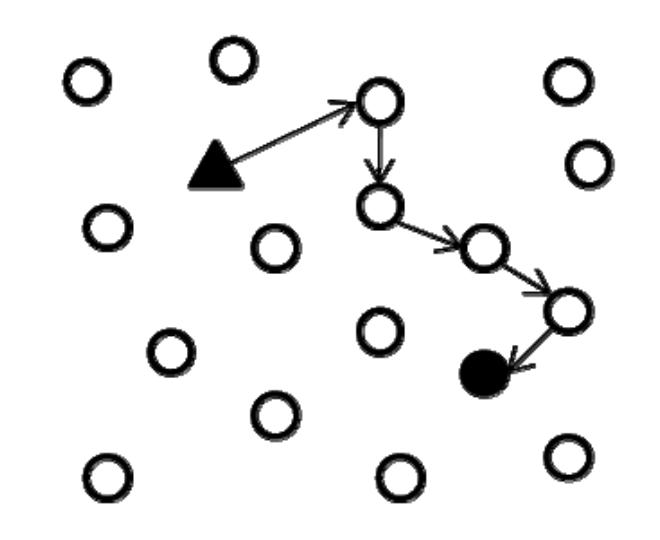
\includegraphics[scale=0.25]{img/orienteering.jpg}
                \end{center}
            \end{column}
        \end{columns}
    }
    \onslide<2->{
        \begin{columns}
            \hspace{0.17cm}
            \begin{column}{0.55\textwidth}
                \begin{block}{Knapsack problem (KP)}
                    \justifying
                    \footnotesize KP is an \textbf{optimization problem} in which the goal is to \textbf{select a subset of items} from a given set such that \textbf{the total value} of the selected items \textbf{is maximized}, while the \textbf{total weight} of the selected items does \textbf{not exceed a given capacity}.
                \end{block}
            \end{column}

            \begin{column}{0.45\textwidth}
                \begin{center}
                    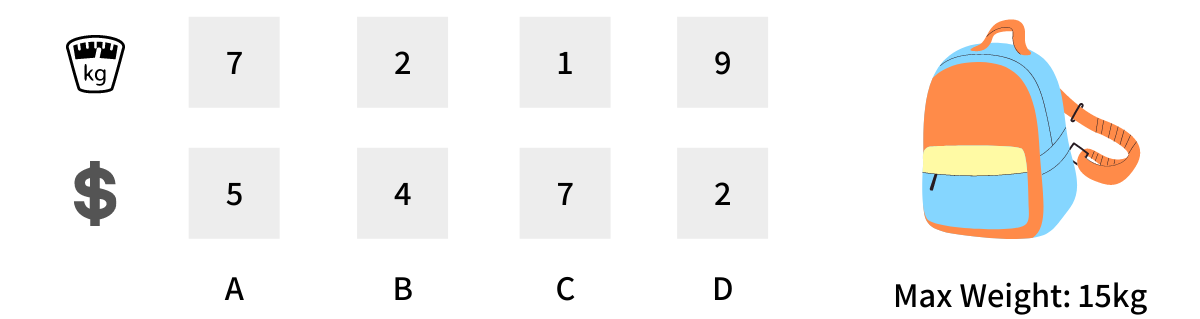
\includegraphics[scale=0.15]{img/knapsack.png}
                \end{center}
            \end{column}
        \end{columns}
    }

\end{frame}

\subsection{Example}
\begin{frame}{Example}
    \begin{columns}
        \begin{column}{0.5\textwidth}
            \begin{center}
                \only<1>{
                    \includesvg[inkscapelatex=false, width=\columnwidth]{img/Example1-v2.svg}
                }
                \only<2>{
                    \includesvg[inkscapelatex=false, width=\columnwidth]{img/Example2-v2.svg}
                }
                \only<3>{
                    \includesvg[inkscapelatex=false, width=\columnwidth]{img/Example3-v2.svg}
                }
                \only<4>{
                    \includesvg[inkscapelatex=false, width=\columnwidth]{img/Example4-v2.svg}
                }
            \end{center}

        \end{column}

        \begin{column}{0.45\textwidth}
            \only<1>{
                \vspace{-5cm}
                \begin{block}{\small Constraints}
                    \footnotesize
                    \begin{itemize}
                        \item $n = 4, m = 5$
                        \item $v_{min} = 0.1, v_{max}  = 1.0, W = 3, T = 75$
                    \end{itemize}

                \end{block}
            }
            \only<2>{

                \begin{block}{\small Constraints}
                    \footnotesize
                    \begin{itemize}
                        \item $n = 4, m = 5$
                        \item $v_{min} = 0.1, v_{max}  = 1.0, W = 3, T = 75$
                    \end{itemize}

                \end{block}
                \begin{block}{\small Solution}
                    \footnotesize
                    \begin{itemize}
                        \item $\pi = \langle 1 \rangle$
                        \item $p = \langle 0, 0, 0 ,0 ,0 \rangle$
                    \end{itemize}
                \end{block}

                \begin{block}{\small Properties}
                    \footnotesize
                    \begin{itemize}
                        \item $p = 0$
                        \item $w = 0$
                        \item $v = v_{max} = 1.0$
                        \item $t = 0$
                    \end{itemize}

                \end{block}
            }

            \only<3>{

                \begin{block}{\small Constraints}
                    \footnotesize
                    \begin{itemize}
                        \item $n = 4, m = 5$
                        \item $v_{min} = 0.1, v_{max}  = 1.0, W = 3, T = 75$
                    \end{itemize}

                \end{block}
                \begin{block}{\small Solution}
                    \footnotesize
                    \begin{itemize}
                        \item $\pi = \langle 1, 3 \rangle$
                        \item $p = \langle 0, 0, 0 ,0 ,0 \rangle$
                    \end{itemize}
                \end{block}

                \begin{block}{\small Properties}
                    \footnotesize
                    \begin{itemize}
                        \item $p = 0$
                        \item $w = 0$
                        \item $v = v_{max} = 1.0$
                              \pause
                        \item $t = d_{1,3} / v = 6 / 1.0 = 6$
                    \end{itemize}

                \end{block}
            }

            \only<4>{

                \begin{block}{\small Constrains}
                    \footnotesize
                    \begin{itemize}
                        \item $n = 4, m = 5$
                        \item $v_{min} = 0.1, v_{max}  = 1.0, W = 3, T = 75$
                    \end{itemize}

                \end{block}
                \begin{block}{\small Solution}
                    \footnotesize
                    \begin{itemize}
                        \item $\pi = \langle 1, 3, 4 \rangle$
                        \item $p = \langle 0, 0, 1 ,0 ,0 \rangle$
                    \end{itemize}
                \end{block}

                \begin{block}{\small Properties}
                    \footnotesize
                    \begin{itemize}
                        \item $p = 100$
                        \item $w = 0 + w_{3} = 3$
                              \pause
                        \item $v = v_{max} - w (v_{max} - v_{min}) / W = 0.1$
                              \pause
                        \item $t = t + d_{3,4} / v = 6 + 5 / 0.1 = 56$
                    \end{itemize}

                \end{block}
            }
        \end{column}
    \end{columns}
\end{frame}

% \subsection{Motivation}
% \begin{frame}{Motivation}
%     \begin{block}{Theoretical Motivation}
%         \vspace{0.2cm}
%         \begin{itemize}
%             \item ThOP can be a benchmark for evaluating and comparing optimization methods.
%             \item ThOP can contribute to solving its component problems OP and KP, even TTP and TSP.
%         \end{itemize}
%         \vspace{0.2cm}
%     \end{block}
%     \pause
%     \begin{block}{Practical Motivation}
%         \vspace{0.2cm}
%         ThOP can be generalized to solve real-world problems:
%         \begin{itemize}
%             \item Planing a route for a vehicle to collect packages in multiple warehouses with time constraints and capacity limits.
%             \item Planing a route for a rescue team to visit a set of locations to collect supplies and rescue victims.
%         \end{itemize}
%         \vspace{0.2cm}
%     \end{block}
% \end{frame}


\subsection{ThOP benchmark}
\begin{frame}{ThOP benchmark}
    \begin{block}{ThOP Benchmark Overview}
        \justifying
        The ThOP benchmark is a collection of 432 instances. Each instance has unique characteristics, including:
        \begin{itemize}
            \item Number of cities: 51, 107, 280, or 1000.
            \item Number of items per city: 01, 03, 05, or 10.
            \item Knapsack types: uncorrelated (unc), uncorrelated with similar weights (usw), or bounded and strongly correlated (bsc).
            \item Knapsack size: 01, 05, or 10 times the size of the smallest knapsack.
            \item Maximum travel time: 50\%, 75\%, or 100\%.
        \end{itemize}
    \end{block}
\end{frame}

\section{Related Works}
\begin{frame}{Related Works}
    \begin{block}{Prior works have proposed various algorithms for ThOP}
        \small
        \begin{itemize}
            % \item Mixed Integer Non-Linear Programming (MINLP)\footnotemark[1]
            \item Iterated local search algorithm (ILS)\footnotemark[1]
            \item Biased random-key genetic algorithm (BRKGA)\footnotemark[1]
            \item Genetic Algorithm (GA)\footnotemark
            \item Ant Colony Optimization algorithm (ACO)\footnotemark
            \item Max-Min Ant System algorithm (ACO++)\footnotemark
        \end{itemize}
    \end{block}
    \footnotetext[2]{\fullcite{9185848}}
    \footnotetext[3]{\fullcite{CHAGAS2020708}}
    \footnotetext[4]{\fullcite{Chagas2021}}
\end{frame}
\section{Previous state-of-the-art method}
\subsection{Max-min ant colony optimization for ThOP}
\begin{frame}{Max-min ant colony optimization for ThOP}
    \begin{columns}
        \begin{column}{0.3\textwidth}
            \begin{center}
                \begin{figure}[htbp]
                    \centering
                    \includesvg[inkscapelatex=false, width=0.9\columnwidth]{img/ACO++.svg}  \\
                    \vspace{0.4cm}
                    \tiny ACO++
                    % \label{fig:aco++fc}
                \end{figure}
            \end{center}
        \end{column}
        \begin{column}{0.5\textwidth}
            \begin{block}{ACO++ overview}
                \footnotesize
                \begin{itemize}
                    \justifying
                    \vspace{0.1cm}
                    \item ACO++, or Max-min Ant Colony Optimization for ThOP, emerged as the state-of-the-art algorithm upon its introduction by its authors.
                          \vspace{0.1cm}
                    \item ACO++ algorithm is a combination of a heuristic approach based on MAX-MIN Ant Colony Optimization with a randomized packing heuristic and local searches.
                          \vspace{0.1cm}
                    \item ACO++ outperformed all other previous algorithms (ACO, BRKGA, ILS, GA) by more than 96\% of the total of test cases.
                          \vspace{0.1cm}
                \end{itemize}
            \end{block}
        \end{column}
    \end{columns}
\end{frame}

\subsection{ACO++'s Randomized Packing Heuristic}
\begin{frame}{ACO++'s Randomized Packing Heuristic}
    \begin{block}{Randomized Packing Heuristic}
        \begin{enumerate}
            \justifying
            \footnotesize
            \item Consider the next item having the highest score.
            \item If picking the item does not violate any constraints, add it to the packing plan.
            \item While items are not all considered, go to step 1.
        \end{enumerate}
    \end{block}
    \pause
    \begin{block}{Item score $s_i$ is determined using the formula}
        \footnotesize
        $$s_i = \frac{p_i^\theta}{w_i^\delta * d_i^\gamma}$$
    \end{block}
    \pause
    \begin{block}{Parameters}
        \begin{itemize}
            \footnotesize
            \justifying
            \item $p_i$: Profit of item $i$.
            \item $w_i$: Weight of item $i$.
            \item $d_i$: Distance from item $i$'s city to the ending city along the route.
            \item $\theta$, $\delta$, $\gamma$: Randomized values within the range [0,1].
        \end{itemize}
    \end{block}
\end{frame}

% \subsection{Adaptive pheromone evaporation}
% \begin{frame}{Adaptive pheromone evaporation}
% \end{frame}


% \subsection{CMA-ES}
% \begin{frame}{CMA-ES}
% \end{frame}


% \subsection{Hierarchical clustering}
% \begin{frame}{Hierarchical clustering}
% \end{frame}


\subsection{Investigating ACO++ Sensitivity to Parameters}
\begin{frame}{Investigating ACO++ Sensitivity to Parameters}
    \begin{block}{The extensive tuning process}
        \begin{itemize}
            \justifying
            \item The ACO++ requires an extensive tuning process to achieve its out-performance results.
            \item The results were obtained using different sets of parameter values that have been extensively fine-tuned for each specific instance group.
        \end{itemize}
        \vspace{0.1cm}
    \end{block}

    \begin{block}{Experiment on ACO++ parameter sensitivity}
        \justifying
        Our experiments were carried out on two instance groups from the ThOP benchmark:
        \begin{itemize}
            \item \texttt{a280\_01\_unc}: 280 cities, 1 item per city, profits uncorrelated with weights.
            \item \texttt{dsj1000\_01\_unc}: 1000 cities, 1 item per city, profits uncorrelated with weights.
        \end{itemize}
        \vspace{0.1cm}
    \end{block}

\end{frame}
\begin{frame}{Investigating ACO++ Sensitivity to Parameters}
    \begin{columns}
        \begin{column}{0.45\textwidth}
            % \begin{block}{Experiments}
            %     \begin{itemize}
            %         \justifying
            %         \footnotesize
            %         \vspace{0.1cm}
            %         \item \textbf{Experiment 1}: Used fine-tuned parameter sets for each instance group.
            %               \vspace{0.1cm}
            %         \item \textbf{Experiment 2}: Swapped parameter sets between instance groups.
            %               \vspace{0.1cm}
            %         \item \textbf{Experiment 3}: Increased $\alpha$, $\beta$, and $\rho$ by 3\% and packing tries by 1.
            %               \vspace{0.1cm}
            %         \item \textbf{Experiment 4}: Used average parameter values from 48 configurations.
            %               \vspace{0.1cm}
            %     \end{itemize}
            \footnotesize
            \begin{block}{Experiment 1}
                Used fine-tuned parameter sets for each instance group.
            \end{block}
            \begin{block}{Experiment 2}
                Swapped parameter sets between instance groups.
            \end{block}
            \begin{block}{Experiment 3}
                Increased $\alpha$, $\beta$, and $\rho$ by 3\% and packing tries by 1.
            \end{block}
            \begin{block}{Experiment 4}
                Used average parameter values from 48 configurations.
            \end{block}
        \end{column}
        \begin{column}{0.45\textwidth}
            % 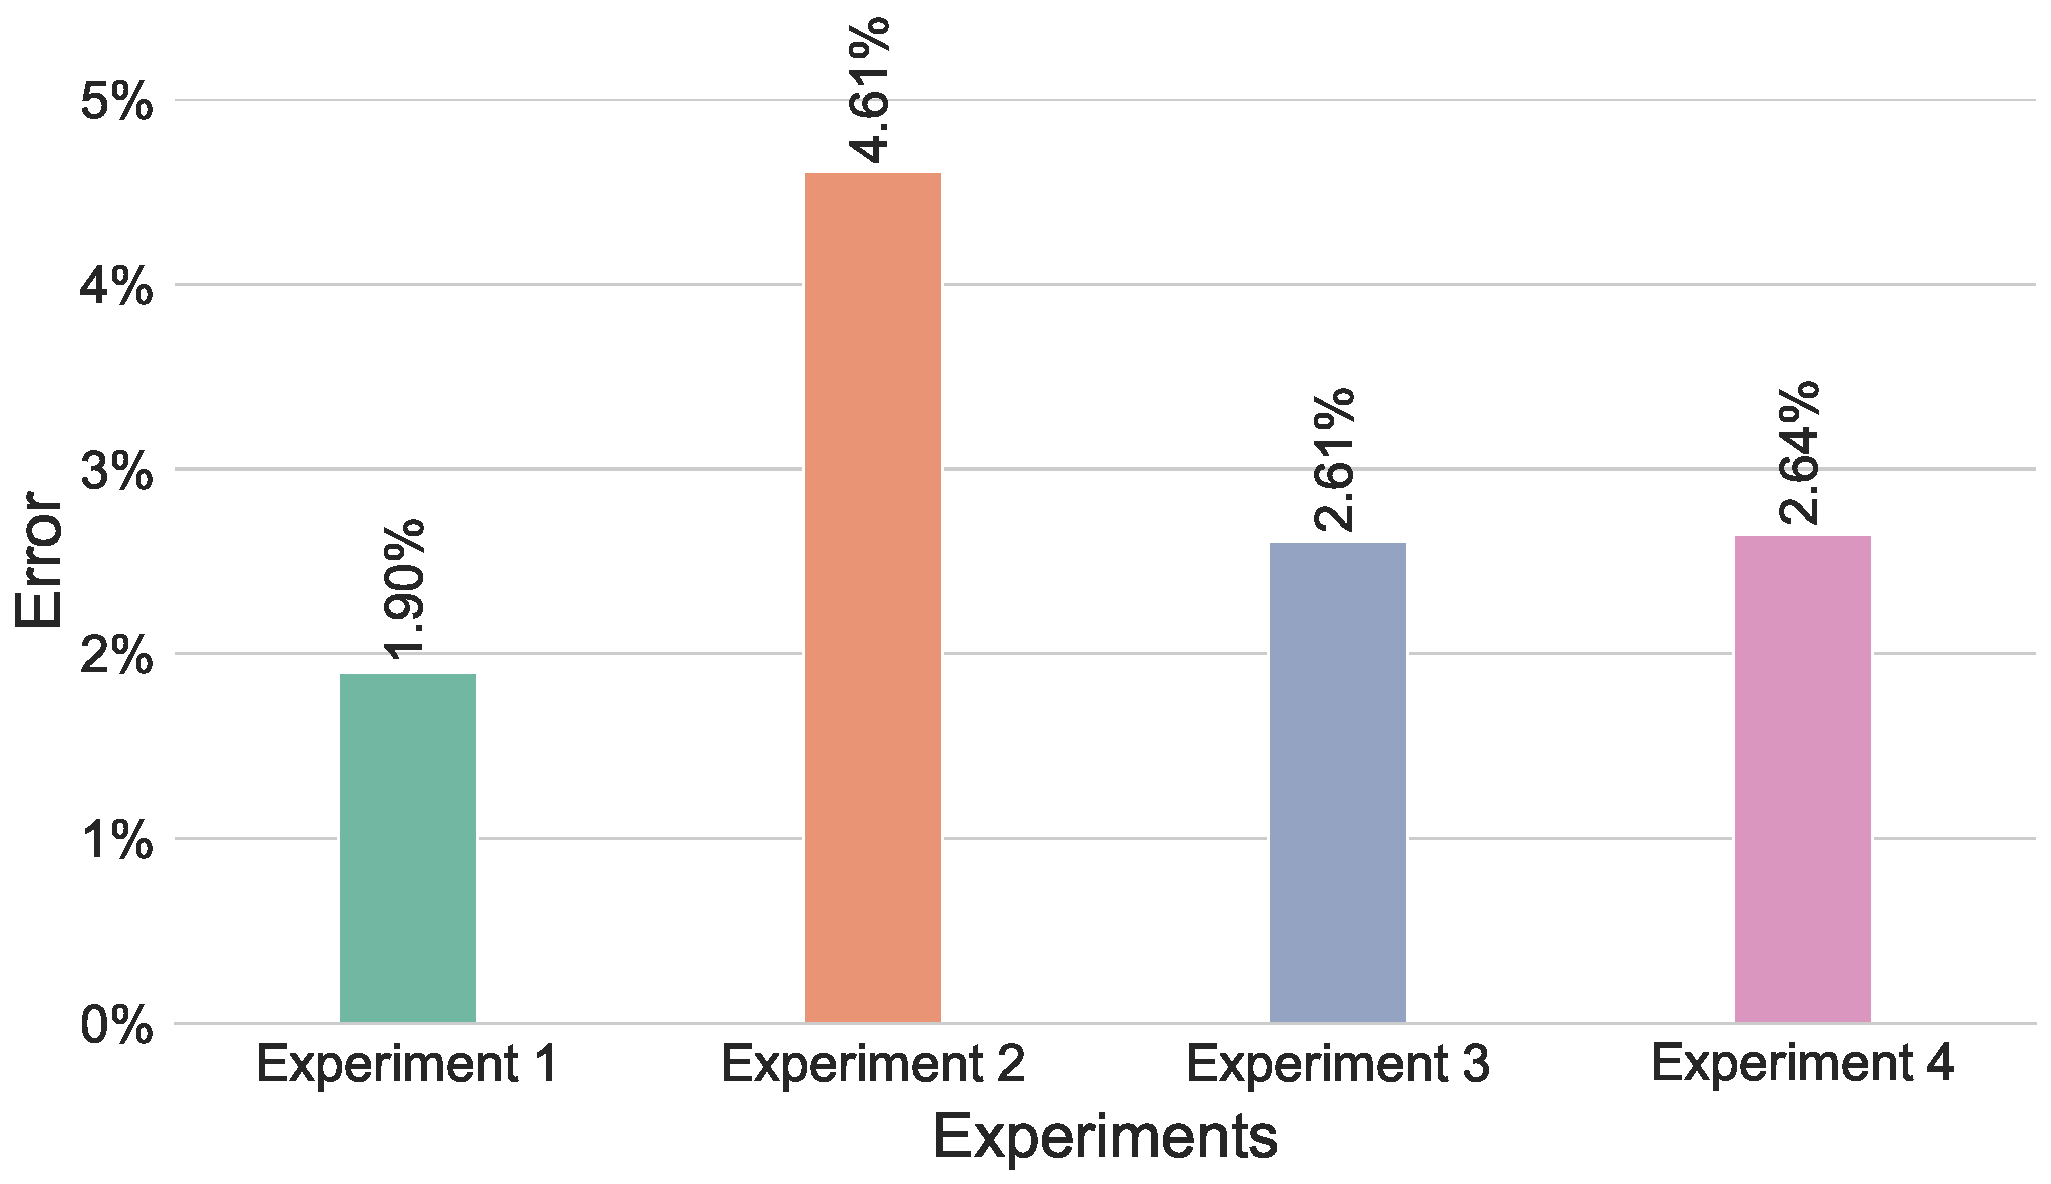
\includegraphics[width=\linewidth]{img/sensitive_error_rate.pdf}
            \begin{figure}[h]
                \centering
                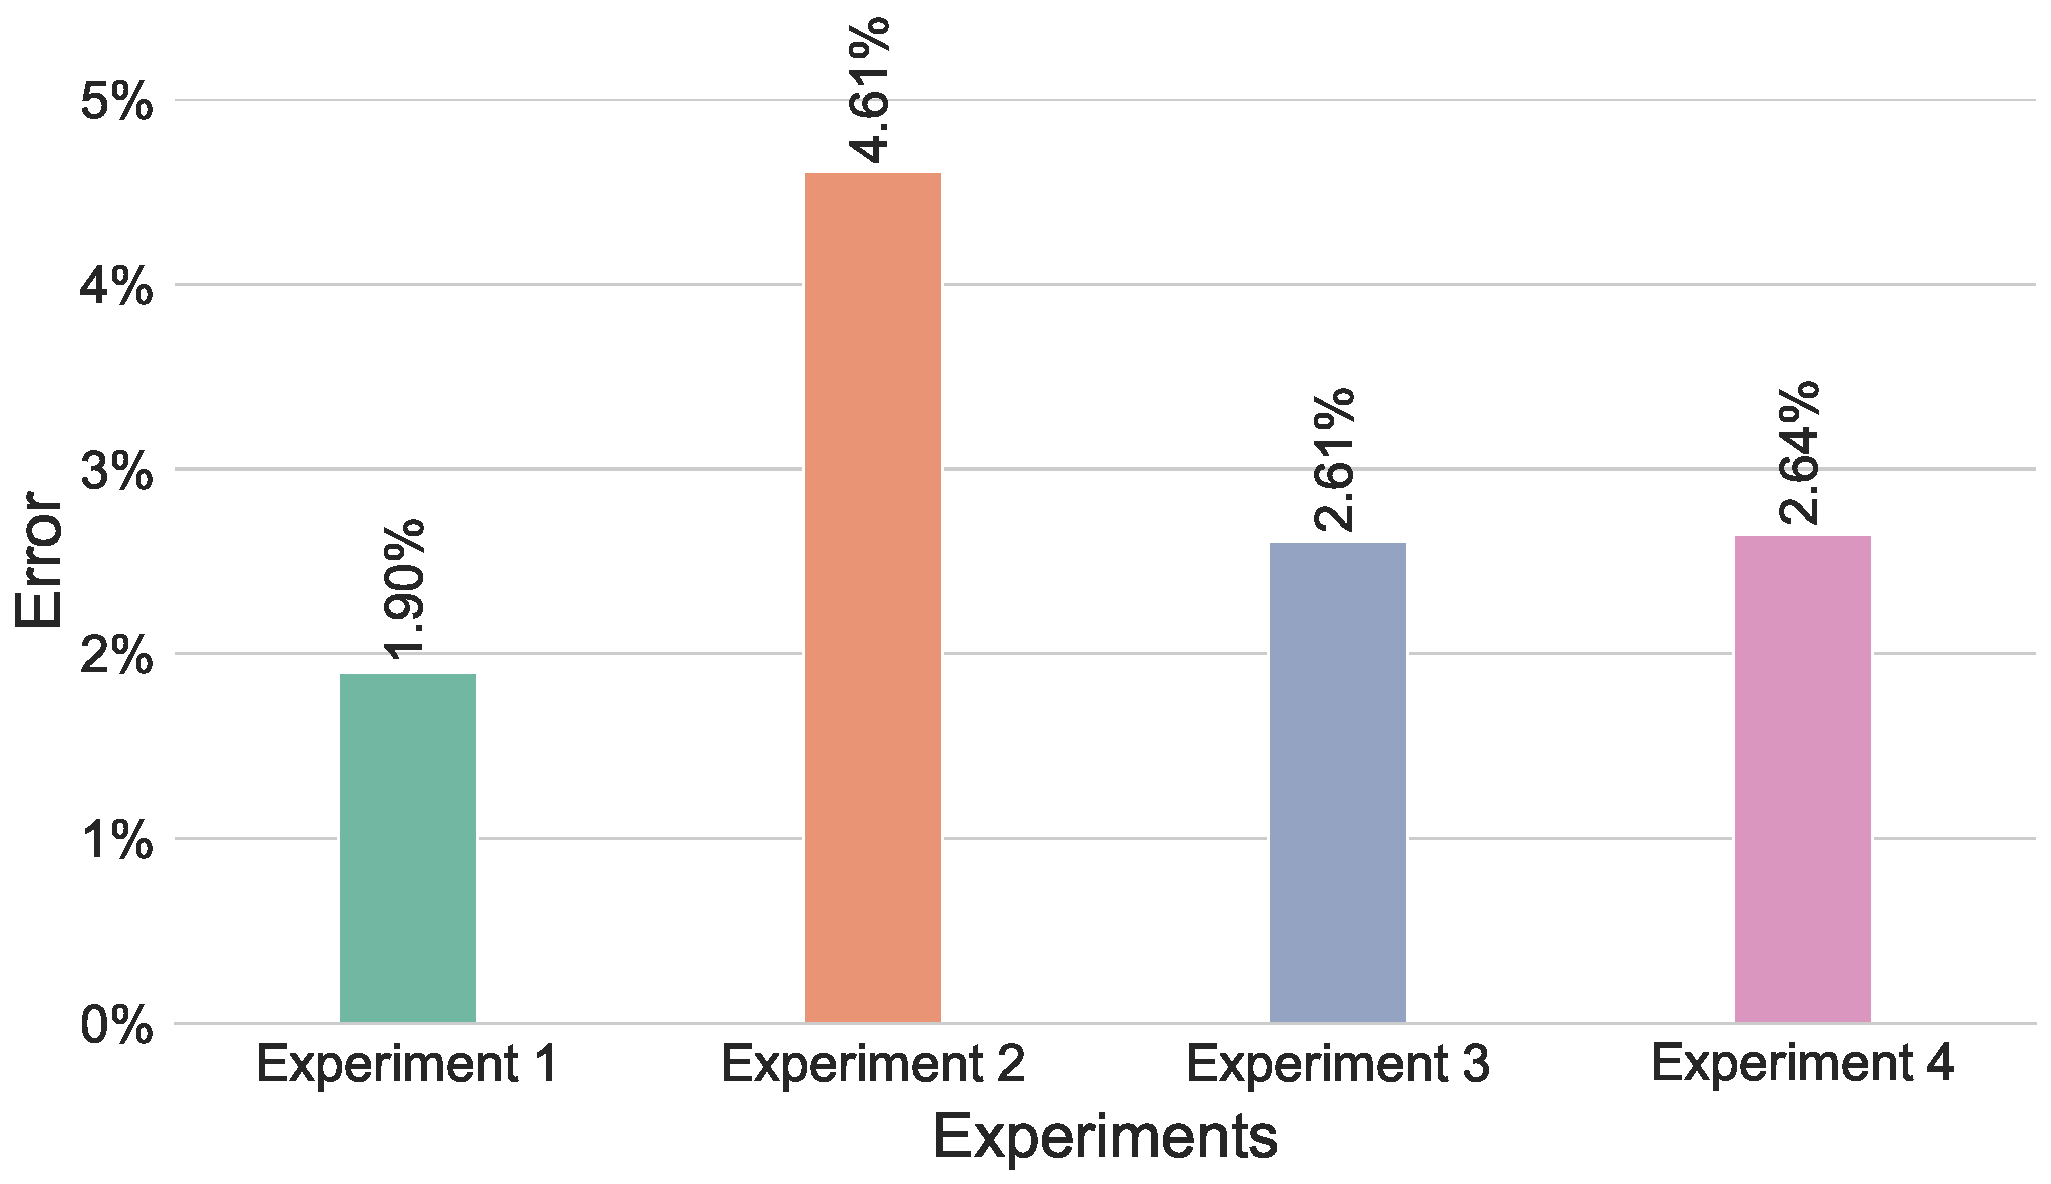
\includegraphics[width=\linewidth]{img/sensitive_error_rate.pdf}
                \caption{\footnotesize Mean errors of results of 4 ACO++ experiments with different parameter sets on 18 instances belonging to 2 ThOP instance groups.}
                % \Description{Mean errors of results of 4 ACO++ experiments with different parameter sets on 2 instance groups.}
                \label{fig:sensitive}
            \end{figure}
        \end{column}
    \end{columns}
\end{frame}
\section{Self-Adaptive Ant System}
\begin{frame}{The overall algorithm}
    \begin{block}{Overview}
        \begin{itemize}
            \justifying
            \vspace{0.1cm}
            \item Our proposed method SAAS, stands for \textbf{S}elf-\textbf{A}daptive \textbf{A}nt \textbf{S}ystem, is an extension of ACO++.
                  \vspace{0.1cm}
            \item It can adapt its parameters based on the ThOP instance and the search process.
                  \vspace{0.1cm}
            \item It also has a lower time complexity in the route-finding and pheromone evaporation phases.
                  \vspace{0.1cm}
        \end{itemize}
    \end{block}
\end{frame}

\begin{frame}{The overall algorithm}
    \vspace{0.1cm}
    \centering
    \includesvg[inkscapelatex=false, width=0.85\columnwidth]{img/SAAS-HC-v3.svg}
\end{frame}


\subsection{Self-adaptive mechanism with CMA-ES}
\begin{frame}{CMA-ES}
    \begin{columns}
        \begin{column}{0.55\textwidth}
            \hspace{0.2cm}
            \begin{block}{Introduction}
                \justifying
                \vspace{0.2cm}
                CMA-ES\footnotemark stands for \textbf{Covariance Matrix Adaptation Evolution Strategy}, which is a \textbf{stochastic}, \textbf{derivative-free} method for numerical optimization of \textbf{non-linear} or \textbf{non-convex} \textbf{continuous} optimization problems. \\
                \vspace{0.2cm}
            \end{block}
        \end{column}

        \begin{column}{0.45\textwidth}
            \vspace{0.1cm}
            \begin{figure}
                \centering
                \includegraphics[width=0.6\columnwidth]{img/simplified_CMA-ES.pdf}
                \footnotesize
                \caption{Simplified CMA-ES.}
            \end{figure}
        \end{column}
    \end{columns}
    \footnotesize \footnotemark[5]{\fullcite{Hansen2006}}
\end{frame}

\begin{frame}{Self-adaptive mechanism with CMA-ES}
    \vspace{0.1cm}
    \centering
    \includesvg[inkscapelatex=false, width=0.85\columnwidth]{img/CMA-ES Flowchart-v3.svg}
\end{frame}


\subsection{Utilizing the profit diversity information for adaptation}
\begin{frame}{Utilizing the profit diversity information for adaptation}
    \vspace{0.1cm}
    \centering
    \includesvg[inkscapelatex=false, width=0.85\columnwidth]{img/Adaptive Flowchart-v3.svg}
\end{frame}

\begin{frame}{Utilizing the profit diversity information for adaptation}
    \begin{block}{Key ideas}
        Inspired by AACO-NC\footnotemark, we use profit diversity information to dynamically change both the number of ants for each ES individual and the pheromone evaporation rate.
        \vspace{0.1cm}
    \end{block}
    \begin{block}{Profit diversity information}
        \begin{equation}\label{eq:entropy_prob}
            p_{i} = \frac{\text{\#occurrences}(P_{i})}{n_{\text{ants}}}
        \end{equation}
        \begin{equation}\label{eq:entropy}
            \begin{split}
                S = \{P\  |\ \text{$P$ is a unique}&\text{ profit value found by the current swarm}\} ,\\
                H &= -\sum_{i=1}^{|S|} p_{i} \cdot \log_2 p_{i}
            \end{split}
        \end{equation}
    \end{block}
    \footnotetext[6]{\fullcite{STODOLA2022101056}}
\end{frame}

\begin{frame}{Utilizing the profit diversity information for adaptation}
    \begin{block}{Adapting the pheromone evaporation rate}
        \vspace{0.1cm}
        \begin{itemize}
            \item The evaporation rate \textbf{increases} for \textbf{high} profit diversity and \textbf{decreases} for \textbf{low} diversity.
        \end{itemize}
        \begin{equation}\label{eq:adaptrho}
            \rho = \rho_{\textbf{min}} \textbf{ + } (\rho_{\text{max}} - \rho_{\text{min}}) \cdot \frac{H - H_{\text{min}}}{H_{\text{max}} - H_{\text{min}}}.
        \end{equation}
        \vspace{0.1cm}
    \end{block}
    \begin{block}{Adapting the number of ants for each ES individual}
        \vspace{0.1cm}
        \begin{itemize}
            \item Unlike the evaporation rate, the value of $n_{\text{indv}}$ \textbf{increases} for \textbf{low} profit diversity to encourage exploration and \textbf{decreases} for \textbf{high} diversity to facilitate exploitation.
        \end{itemize}
        \begin{equation} \label{eq:adaptants}
            n_{\text{indv}} = n_{\text{indv\_}\textbf{max}} \textbf{ - } (n_{\text{indv\_max}} - n_{\text{indv\_min}}) \cdot \frac{H - H_{\text{min}}}{H_{\text{max}} - H_{\text{min}}}.
        \end{equation}
        \vspace{0.1cm}
    \end{block}
\end{frame}


\begin{frame}{Parameters controlled}
    \begin{table}
        \small
        \caption{List of Parameters controlled by Parameter Control Mechanisms}
        \label{tab:control_param}
        \begin{tabular}{l|l|l}
            \hline
            Parameter                                & Parameter control mechanism & Range                                            \\
            \hline
            % $n\_ants$                   &   adaptive                    \\
            $\alpha$                                 & Self-adaptive               & [0, 1]                                           \\
            $\beta$                                  & Self-adaptive               & [0, 1]                                           \\
            $\rho_{\text{min}}$, $\rho_{\text{max}}$ & Self-adaptive               & [0, 1]                                           \\
            $\theta$                                 & Self-adaptive               & [0, 1]                                           \\
            $\delta$                                 & Self-adaptive               & [0, 1]                                           \\
            $\gamma$                                 & Self-adaptive               & [0, 1]                                           \\
            $n_{\text{indv}}$                        & Adaptive                    & [$n_{\text{indv\_max}}$, $n_{\text{indv\_min}}$] \\
            $\rho$                                   & Adaptive                    & [$\rho_{\text{min}}, \rho_\text{{max}}$]         \\
            \hline
        \end{tabular}
    \end{table}
\end{frame}


\subsection{Ant traversal on cluster trees}
\begin{frame}{Ant traversal on cluster trees}
    \vspace{0.1cm}
    \centering
    \includesvg[inkscapelatex=false, width=0.85\columnwidth]{img/Tree Flowchart-v3.svg}
\end{frame}

\begin{frame}{Ant traversal on cluster trees}
    \begin{columns}
        \begin{column}{0.55\textwidth}
            \begin{block}{Key ideas}
                \vspace{0.1cm}
                \begin{itemize}
                    \justifying
                    \item We use hierarchical clustering to build the tree architecture.
                    \item Each city has its own cluster tree that represents the edges going to $n$ cities.
                    \item Ants will traverse cluster trees instead of moving directly from one city to another.
                    \item This way, we can reduce the time complexity of choosing the next city to $\Theta(\log n)$.
                \end{itemize}
                \vspace{0.1cm}
            \end{block}
        \end{column}
        \begin{column}{0.45\textwidth}
            \begin{figure}
                \vspace{0.1cm}
                \centering
                \includesvg[inkscapelatex=false, width=0.85\columnwidth]{img/Cluster tree-v2.svg}
                \footnotesize \caption{Cluster tree example.}
            \end{figure}
        \end{column}
    \end{columns}
\end{frame}


\subsection{Lazy evaporation}
\begin{frame}{Lazy evaporation}
    \vspace{0.1cm}
    \centering
    \includesvg[inkscapelatex=false, width=0.85\columnwidth]{img/Lazy-v3.svg}
\end{frame}

\begin{frame}{Lazy evaporation}
    \begin{block}{Key ideas}
        \begin{itemize}
            \justifying
            \vspace{0.1cm}
            \item The key idea of lazy evaporation is to keep track of historical and desired states.
                  \vspace{0.1cm}
            \item The desired state consists of the number of times that pheromones need evaporating.
                  \vspace{0.1cm}
            \item Each edge has its historical state including the number of times that the pheromone of the edge has been evaporated.
                  \vspace{0.1cm}
            \item By comparing historical states and the desired state, we can determine how to calculate the desired pheromones of edges when needed.
                  \vspace{0.1cm}
        \end{itemize}
    \end{block}
\end{frame}


% \begin{frame}{Lazy evaporation}
% \begin{block}{Parameters}

% \end{block}

% \begin{block}{Calculate true pheromone}
% \begin{itemize}
%     \item $\tau_\text{true} \gets \tau_\text{local} \times (1-\rho)^{\text{GECount} - \text{LECount}}$
% \end{itemize}
% \end{block}

% \begin{block}{Evaporate pheromonCommunication}
% \begin{itemize}
%     \item $\text{GECount} \gets \text{GECount} + 1$
% \end{itemize}
% \end{block}

% \begin{block}{Deposit pheromone}
% \begin{itemize}
%     \item $\tau_\text{local} \gets \tau_\text{true} + \Delta\tau$
%     \item $\text{LECount} \gets \text{GECount}$
% \end{itemize}
% \end{block}
% \end{frame}


\begin{frame}{The overall algorithm}
    \vspace{0.1cm}
    \centering
    \includesvg[inkscapelatex=false, width=0.85\columnwidth]{img/SAAS-HC-v3.svg}
\end{frame}

\section{Experiments}
\begin{frame}{Experiments}
    \begin{block}{Hardware}
        Experiments were run on the same machine with Intel(R) Core(TM) i7-8750H @ 2.20GHz for a fair comparison.
    \end{block}
    \begin{block}{Hyperparameter tuning}
        \begin{itemize}
            \item BRKGA, ACO, and ACO++ used the same parameters fine-tuned in the ACO++ paper.
            \item 240,000 experiments were performed for tuning each algorithm. ILS had no parameters to fine-tune.
            \item evosax\footnotemark framework was used to tune SAAS hyperparameters.
            \item 45,000 experiments were performed to tune SAAS for all benchmark instances.
        \end{itemize}
    \end{block}
    \footnotetext[7]{\fullcite{lange2022evosax}}
\end{frame}
% \subsection{Approximation ratio of the solution approaches}
\begin{frame}{Approximation ratio of the solution approaches}
    \centering
    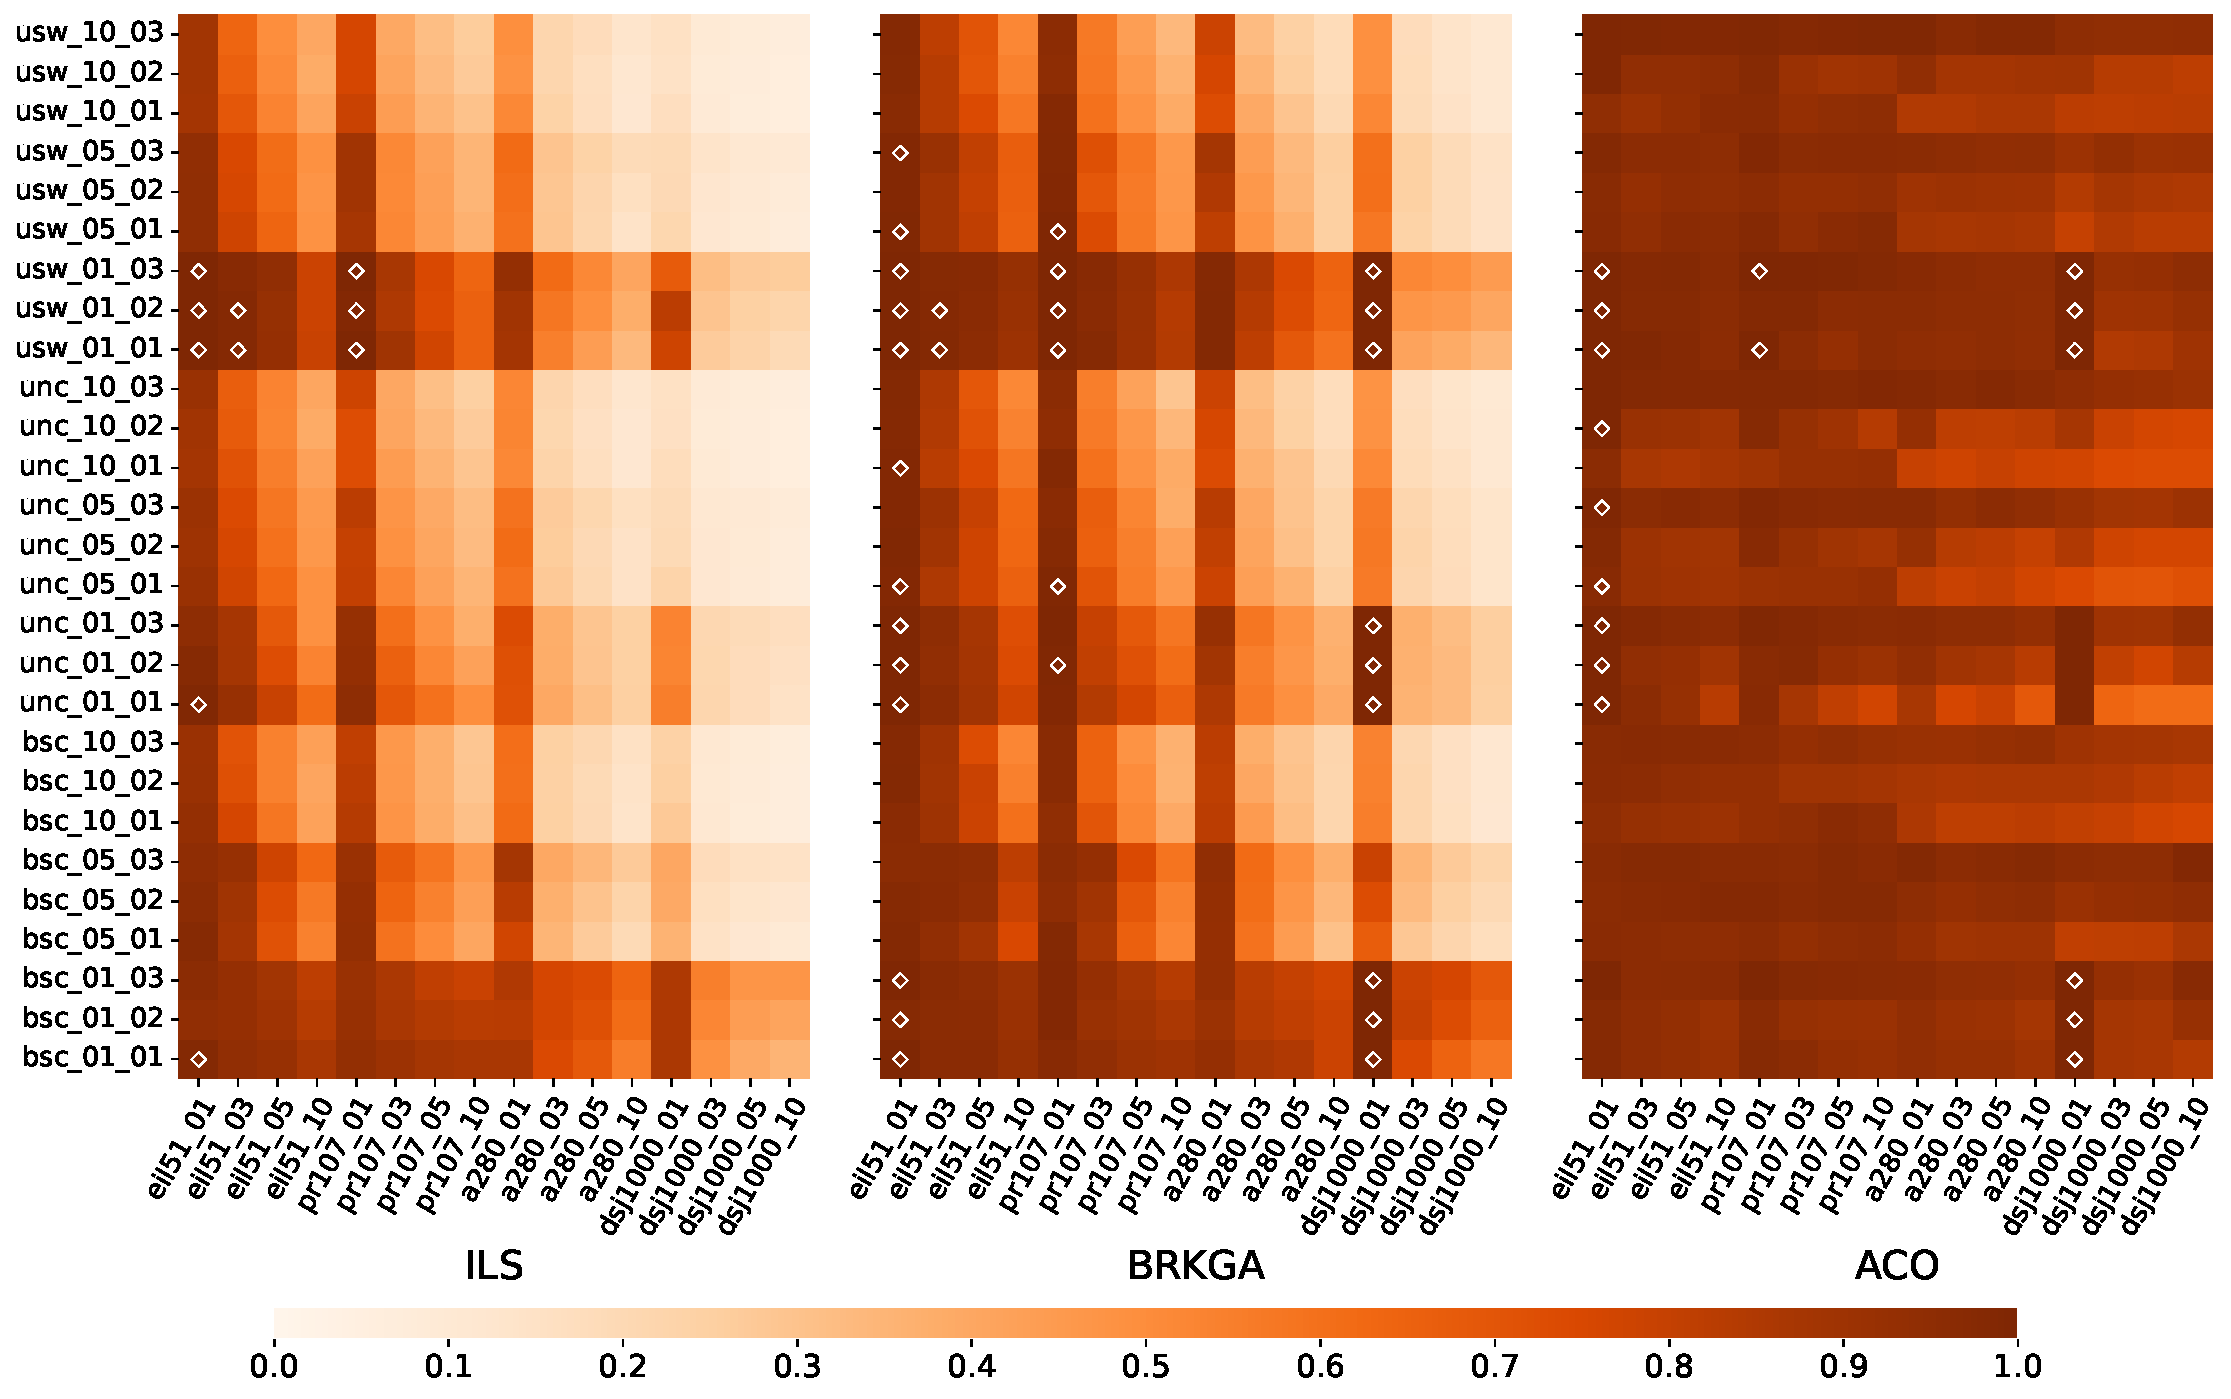
\includegraphics[width=0.7\linewidth]{img/profit_ratio_horizontal_1.pdf}
\end{frame}
\begin{frame}{Approximation ratio of the solution approaches}
    \centering
    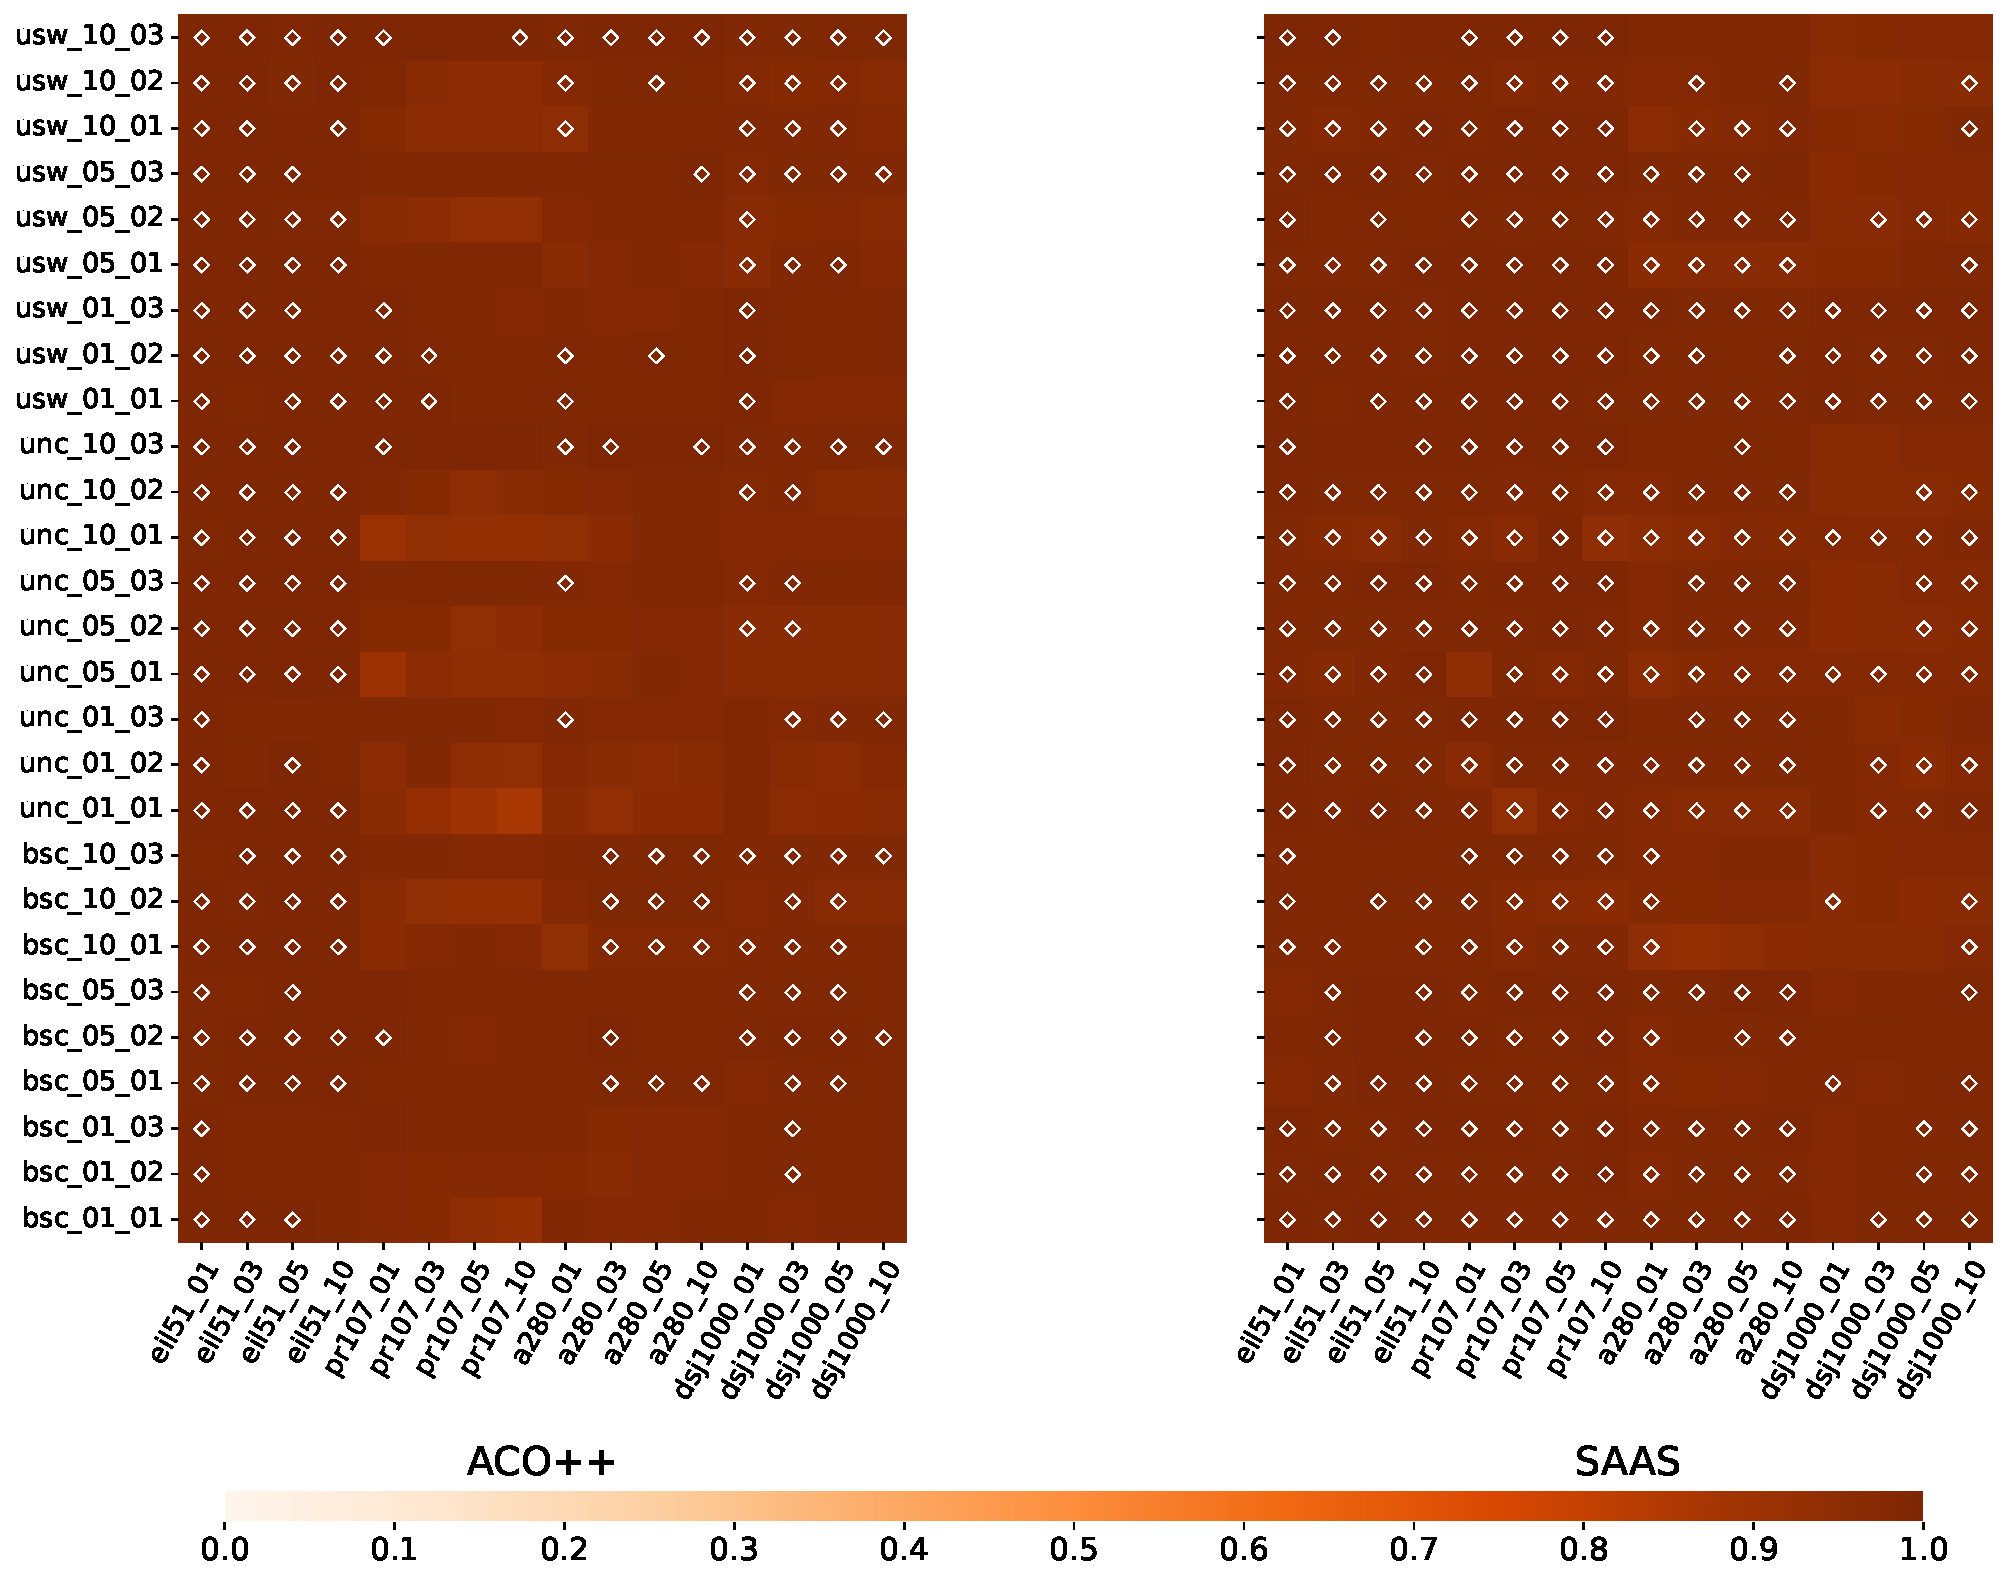
\includegraphics[width=0.6\linewidth]{img/profit_ratio_horizontal_2.pdf}
\end{frame}
% \subsection{Comparing performance between algorithms}
\begin{frame}{Comparing performance between algorithms}
    \centering
    \begin{table}
        \small
        \caption{Percentage of the number of instances in which algorithm i found better or equal quality solutions than algorithm j}
        \label{tab:winpercent}
        \begin{tabular}{l|rrrrr}
            \hline
            i $\downarrow$ \ \ \ \ j $\rightarrow$ & ILS      & BRKGA   & ACO     & ACO++   & SAAS    \\
            \hline
            ILS                                    & -        & 2.55\%  & 4.40\%  & 2.55\%  & 2.31\%  \\
            BRKGA                                  & 100.00\% & -       & 16.20\% & 8.80\%  & 7.18\%  \\
            ACO                                    & 97.22\%  & 87.27\% & -       & 5.79\%  & 4.86\%  \\
            ACO++                                  & 99.54\%  & 95.83\% & 97.69\% & -       & 41.90\% \\
            SAAS                                   & 99.77\%  & 97.92\% & 98.61\% & 78.24\% & -       \\
            \hline
        \end{tabular}
    \end{table}
\end{frame}
% \subsection{Error rate of SAAS solutions}
\begin{frame}{Error rate of SAAS solutions}
    \begin{figure}
        \centering
        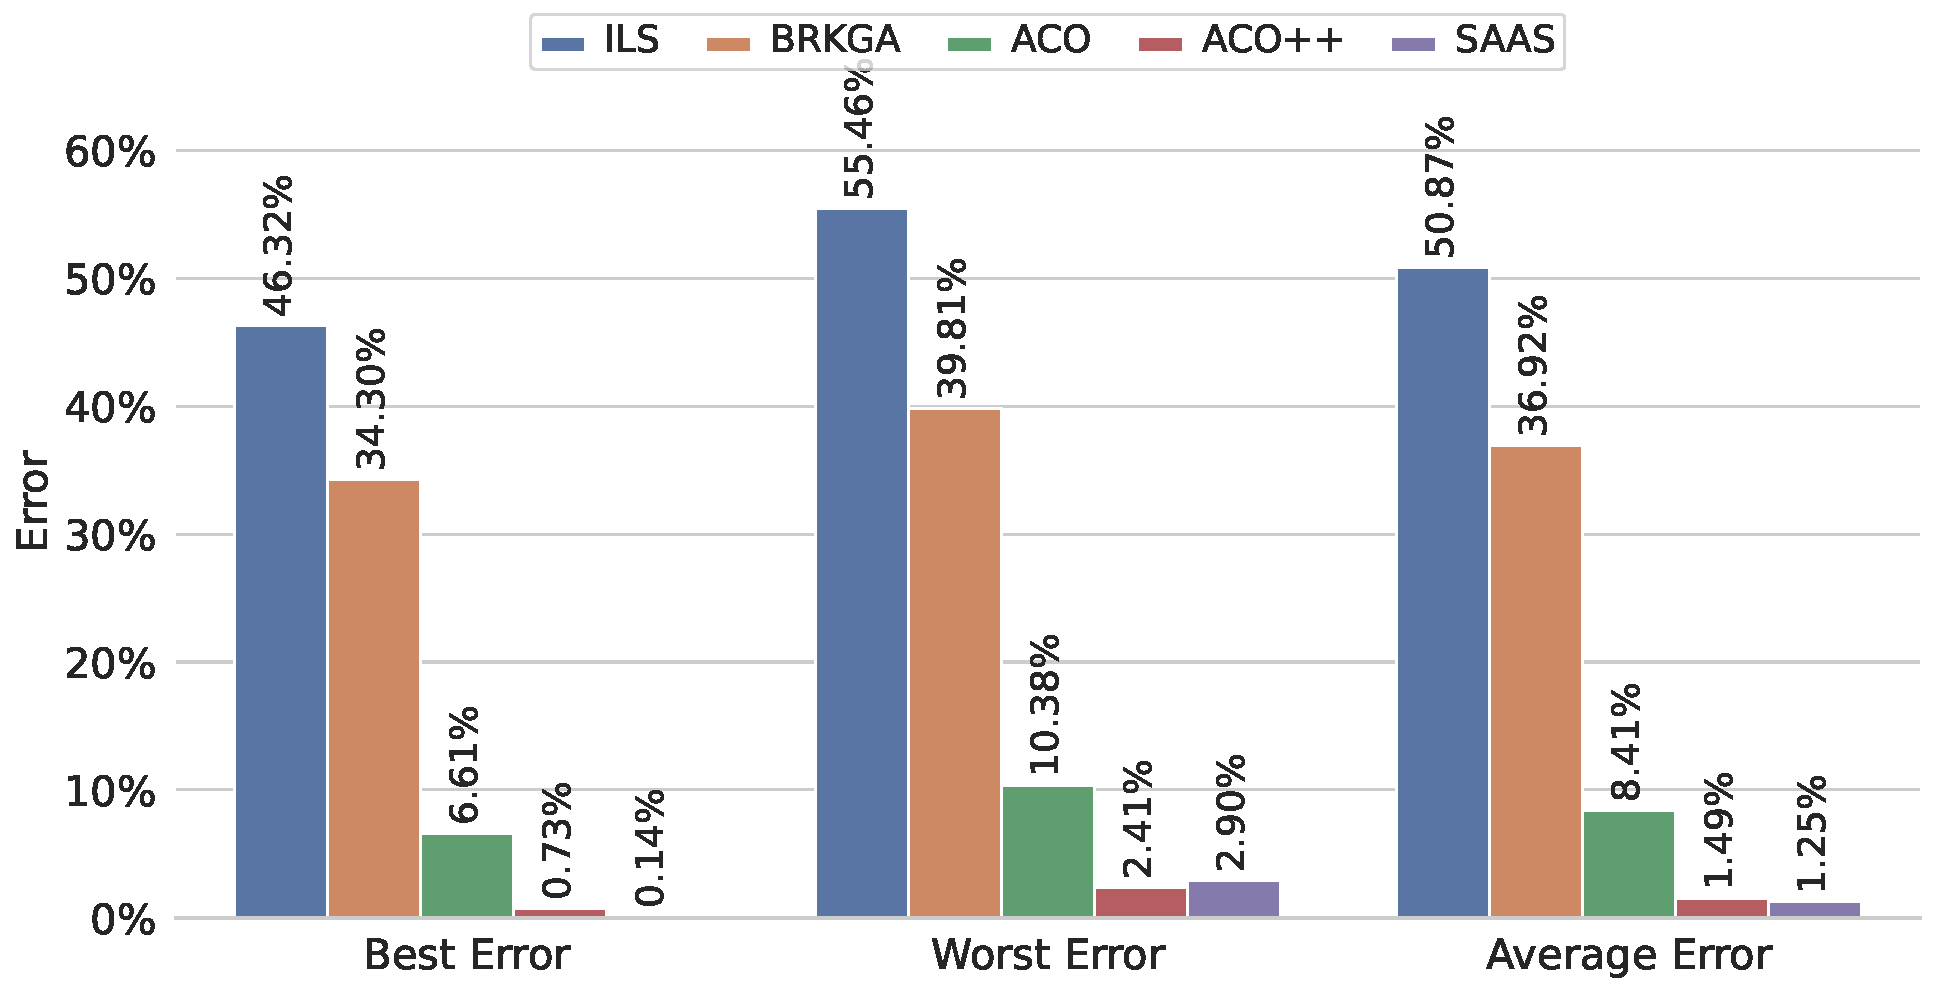
\includegraphics[width=0.75\linewidth]{img/error_rate.pdf}
        \caption{Mean errors overall benchmark instances.}
        % \Description{Mean errors over all benchmark instances.}
        \label{fig:error_rate}
    \end{figure}
\end{frame}
\section{Conclusion}
\begin{frame}{Conclusion}
    \begin{block}{Conclusion}
        \begin{itemize}
            \justifying
            \item Parameter control mechanisms are incorporated to improve adaptability and flexibility.
            \item Lazy evaporation technique is used to reduce the time complexity of the evaporation phase.
            \item Hierarchical clustering is used to improve the time complexity of finding routes.
            \item SAAS is more efficient than ACO++ and requires only one hyperparameter set to run all 432 benchmark instances.
            \item  The SAAS algorithm showcases remarkable performance when it surpasses all other algorithms for ThOP.
        \end{itemize}
        \vspace{0.1cm}
    \end{block}
\end{frame}
\begin{frame}{References}
    \printbibliography
\end{frame}
\end{document}
